\taskpic{При слабом ударе футбольного мяча о стенку он деформируется
  как показано на рисунке. При этом деформация мяча $x$ много меньше
  его радиуса и можно считать, что давление $p$ воздуха в мяче в
  процессе удара не меняется. Пренебрегая упругостью покрышки, оценить
  время соударения мяча со стеной. Провести числовой расчет этого
  времени для случая, когда масса мяча $m = 0.5$~кг, давление в нем
  $p$ = $2 \cdot 10^5$~Па, и радиус мяча $R = 12.5$~см.}{%
  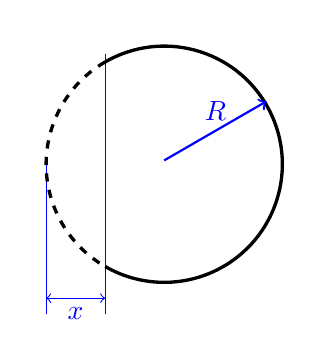
\begin{tikzpicture}
    \draw[blue] (2,2.1) -- (2,-1.2);
    \draw[blue] (1.25,0.75) -- (1.25,-1.2);
    \draw[very thick] (2cm,2cm) arc (120:-120:1.5cm);
    \draw[very thick,dashed] (2cm,2cm) arc (120:240:1.5cm);
    \draw[blue,<->] (1.25,-1) -- (2,-1) node[below,midway] {$x$};
    \draw[blue,thick,->] (2.75,0.75) -- ++(30:1.5cm) node[right,above,midway] {$R$};
  \end{tikzpicture}
}
